\documentclass{beamer}
\usepackage{graphicx}
\usepackage{listings}
\usepackage{ulem}

\usetheme{Dresden}
\setbeamertemplate{navigation symbols}{}

\usepackage{mathtools}
\newcommand{\dd}{\, \text{d}}
\renewcommand{\vec}[1]{\ensuremath{\mathbf{#1}}}
\newcommand{\mat}[1]{\ensuremath{\mathbf{#1}}}
\newcommand{\op}[1]{\ensuremath{\mathbf{#1}}}
\newcommand{\norm}{\ensuremath{\mathcal{N}}}

\usepackage{algorithm}
\usepackage{algpseudocode}

\title[HMC]{Implementing Hamiltonian Monte Carlo for Efficent Bayesian Evolutionary Analysis}
\author{Arman Bilge}
\date{2nd April 2015}

\begin{document}

    \frame{\titlepage}

    \section{Introduction}

    \begin{frame}{What is Bayesian Evolutionary Analysis?}

        Problems which are centered around sampling from the posterior distribution of trees given sequence data, given by

        \begin{equation*}
            p\left(T \mid D\right)
                \propto \int_\theta p\left(D \mid T,\theta\right)
                p\left(T \mid \theta\right) p\left(\theta\right) \dd\theta,
        \end{equation*}

        where \\
        $p\left(D \mid T,\theta\right)$ is the Felsenstein tree likelihood, \\
        $p\left(T \mid \theta\right)$ is the tree prior, and \\
        $\theta$ are nuisance parameters.

        \vspace{14pt}
        Markov chain Monte Carlo samplers have been successfully applied to these distributions.
        Because samples are inherently correlated, we aim to maximise the effective sample size (ESS).

    \end{frame}

    \begin{frame}{Bayesian Evolutionary Analysis using MCMC}

        \begin{itemize}
            \item \only<1>{We are very good at creating a Markov chain that converges to the target distribution.} \only<2->{\sout{We are very good at creating a Markov chain that converges to the target distribution.}}
            \item<2-> We are very good at coercing just about any old Markov chain to converge to the target distribution via Metropolis--Hastings:
            \begin{equation*}
                a = \min\left(1, \frac{\pi\left(q^\prime\right)T\left(q^\prime\to q\right)}{\pi\left(q\right)T\left(q\to q^\prime\right)}\right)
            \end{equation*}
            \pause
            \item Hence, chain is generally driven by a na\"ive set of operators.
        \end{itemize}

    \end{frame}

    \begin{frame}{Properties of MCMC}

        \begin{itemize}
            \item Ergodicity depends on the proposal distribution
            \item Optimal proposal acceptance rate is $0.234$
            \item Scales on the order of $d^2$ thanks to random walk
            \item Difficult to update multiple parameters at once
            \item Difficult to make distant proposals that will be accepted
            \item We can do better!
        \end{itemize}

    \end{frame}

    \section{Theory}

    \begin{frame}{Hamiltonian Dynamics}
        \begin{definition}
            Let $\pi\left(\vec{q}\right)$ be the target probability density.
            Consider a particle of mass~$\mat{M}$ in the state space.
            We augment its position $\vec{q}$ with momentum $\vec{p}$ and define
            the \emph{Hamiltonian} for our system as
            \begin{equation*}
                H\left(\vec{q},\vec{p}\right) = U\left(\vec{q}\right) + K\left(\vec{p}\right)
            \end{equation*}
            with potential energy
            \begin{equation*}
                U\left(\vec{q}\right) = - \log{\pi\left(\vec{q}\right)}
            \end{equation*}
            and kinetic energy
            \begin{equation*}
                K\left(\vec{p}\right) = \frac{1}{2} \vec{p}^T \mat{M}^{-1} \vec{p}
            \end{equation*}
            % Consider a particle. Let its position $\vec{q}$ be the parameter of interest and momentum $\vec{p}$ be an auxillary parameter.
        \end{definition}

    \end{frame}

    \begin{frame}{Hamiltonian Dynamics}

        The dynamics of this system are given by Hamilton's equations
            \begin{align*}
                \frac{\dd \vec{q}}{\dd t} &= \frac{\partial H}{\partial \vec{p}} \\
                \frac{\dd \vec{p}}{\dd t} &= -\frac{\partial H}{\partial \vec{q}}
            \end{align*}
        which can be integrated to map the particle's state from one point in time to another.

    \end{frame}

    \begin{frame}{Properties of Hamiltonian Dynamics}
        \begin{itemize}
            \item Reversibility
            \item Energy-conservation
            \item Volume-preservation (symplecticness)
        \end{itemize}
    \end{frame}

    \begin{frame}{The Operations}

        \begin{definition}
            $\op{L}\left\{\vec{q},\vec{p}\right\}$ maps the state at time~$t$ to the state at time~$t + \epsilon L$, as approximated by $L$~leapfrog steps of size~$\epsilon$.
        \end{definition}

        \vfill

        \centering
        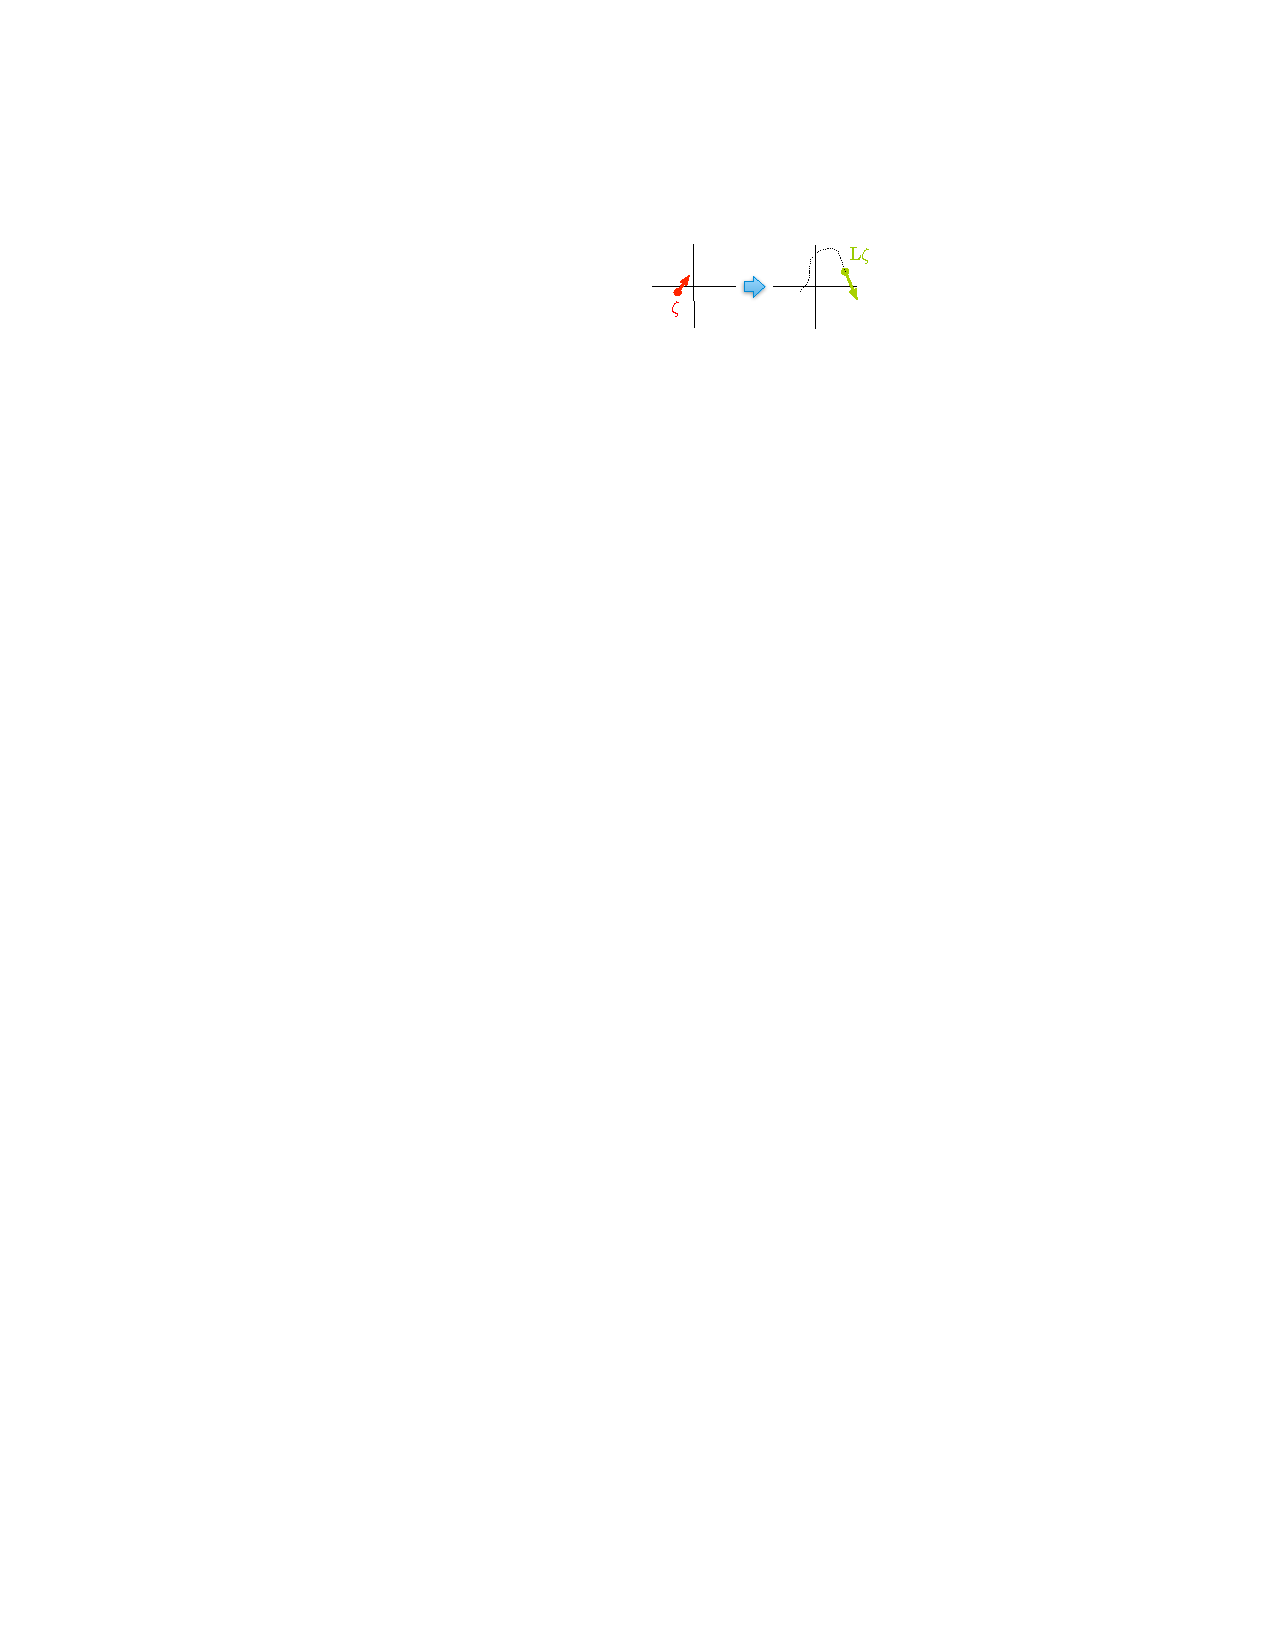
\includegraphics[width=0.75\textwidth]{L.pdf}

    \end{frame}

    \begin{frame}{The Leapfrog Integrator}

        \begin{block}{A single leapfrog step}
            \begin{equation*}
                \vec{p}\left(t+\frac{\epsilon}{2}\right) = \vec{p}\left(t\right) - \frac{\epsilon}{2} \cdot \frac{\partial U}{\partial \vec{q}} \odot \vec{q}\left(t\right)
            \end{equation*}
            \pause
            \begin{equation*}
                \vec{q}\left(t+\epsilon\right) = \vec{q}\left(t\right) + \epsilon \cdot \frac{\partial K}{\partial \vec{p}} \odot \vec{p}\left(t+\frac{\epsilon}{2}\right)
            \end{equation*}
            \pause
            \begin{equation*}
                \vec{p}\left(t+\epsilon\right) = \vec{p}\left(t + \frac{\epsilon}{2}\right) - \frac{\epsilon}{2} \cdot \frac{\partial U}{\partial \vec{q}} \odot \vec{q}\left(t+\epsilon\right)
            \end{equation*}
        \end{block}

        The leapfrog method is a symplectic integrator appropriate for Hamiltonian dynamics.

    \end{frame}

    \begin{frame}{The Operations}

        \begin{definition}
            $\op{F}\left\{\vec{q},\vec{p}\right\} = \left\{\vec{q},-\vec{p}\right\}$ flips the momentum.
        \end{definition}

        \vfill

        \centering
        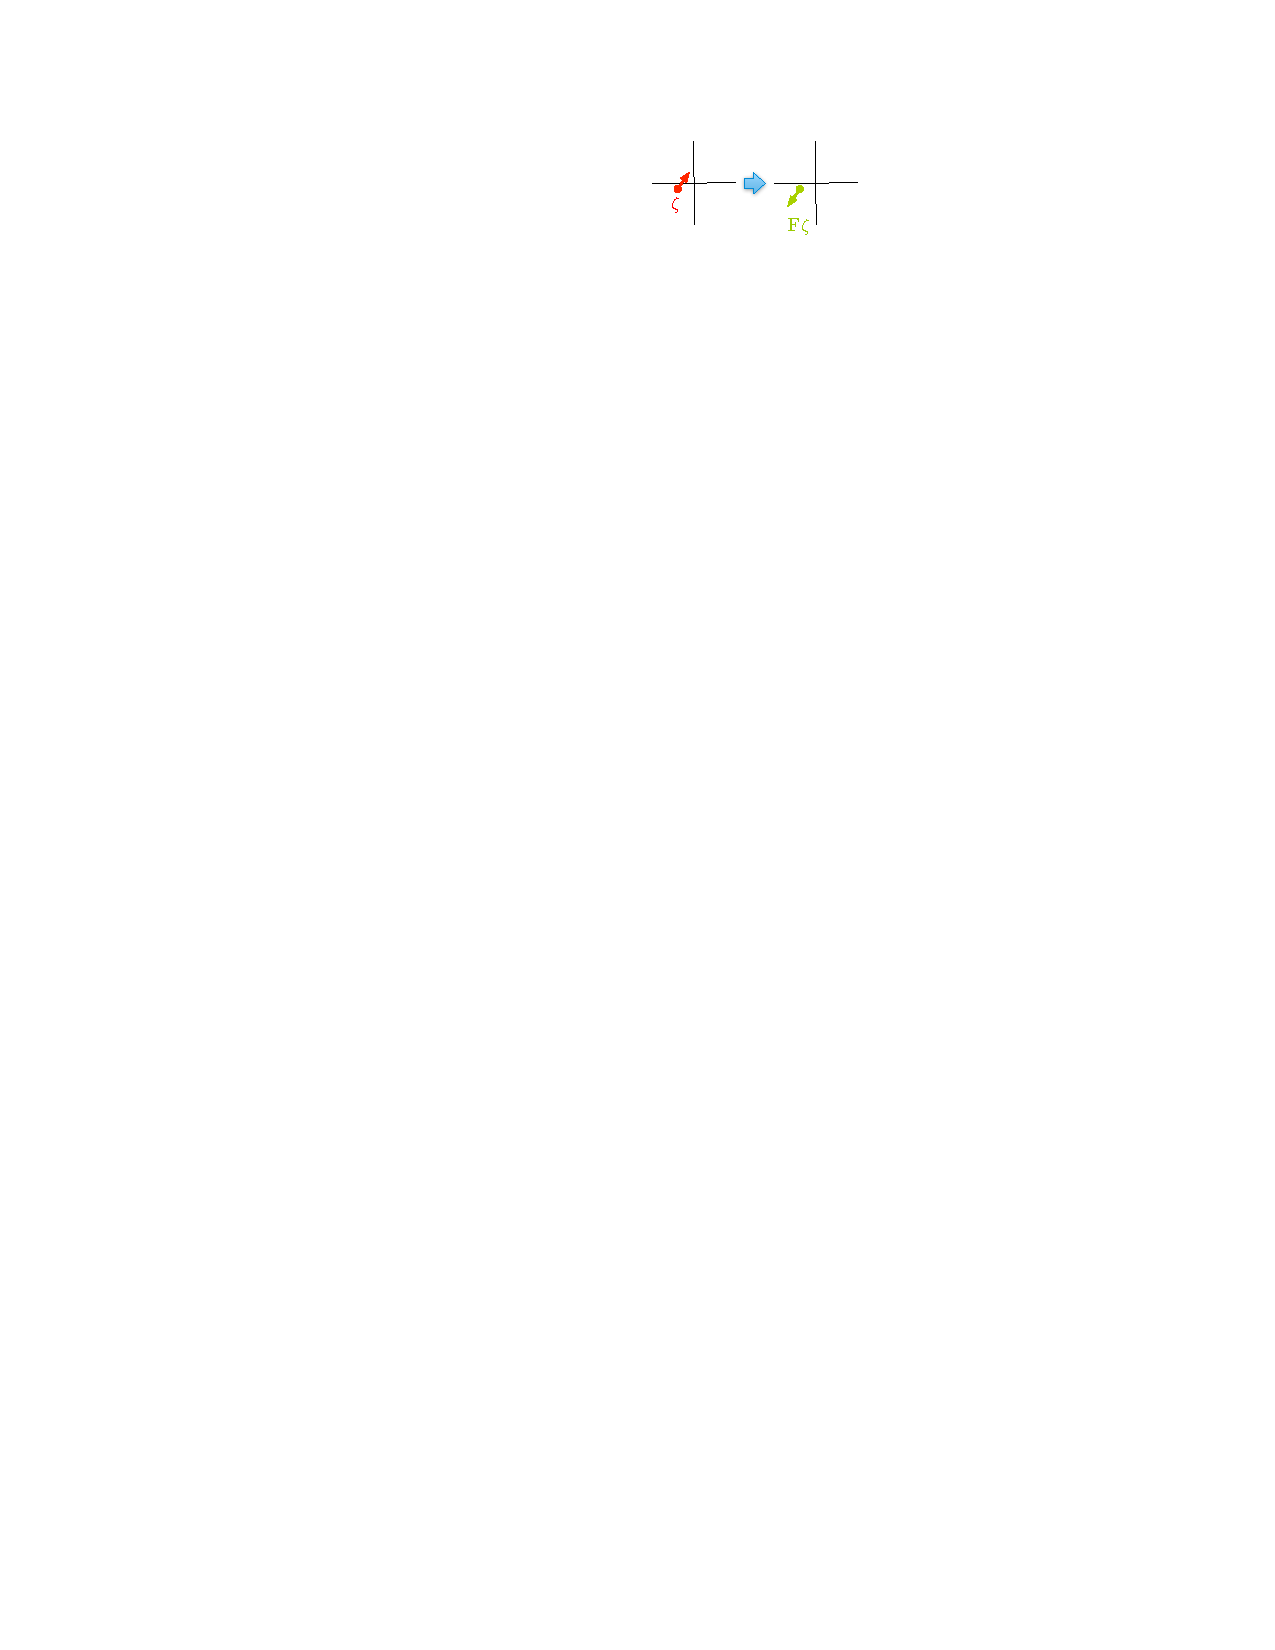
\includegraphics[width=0.75\textwidth]{F.pdf}

    \end{frame}

    \begin{frame}{Discrete Ladder of HMC}
        \centering
        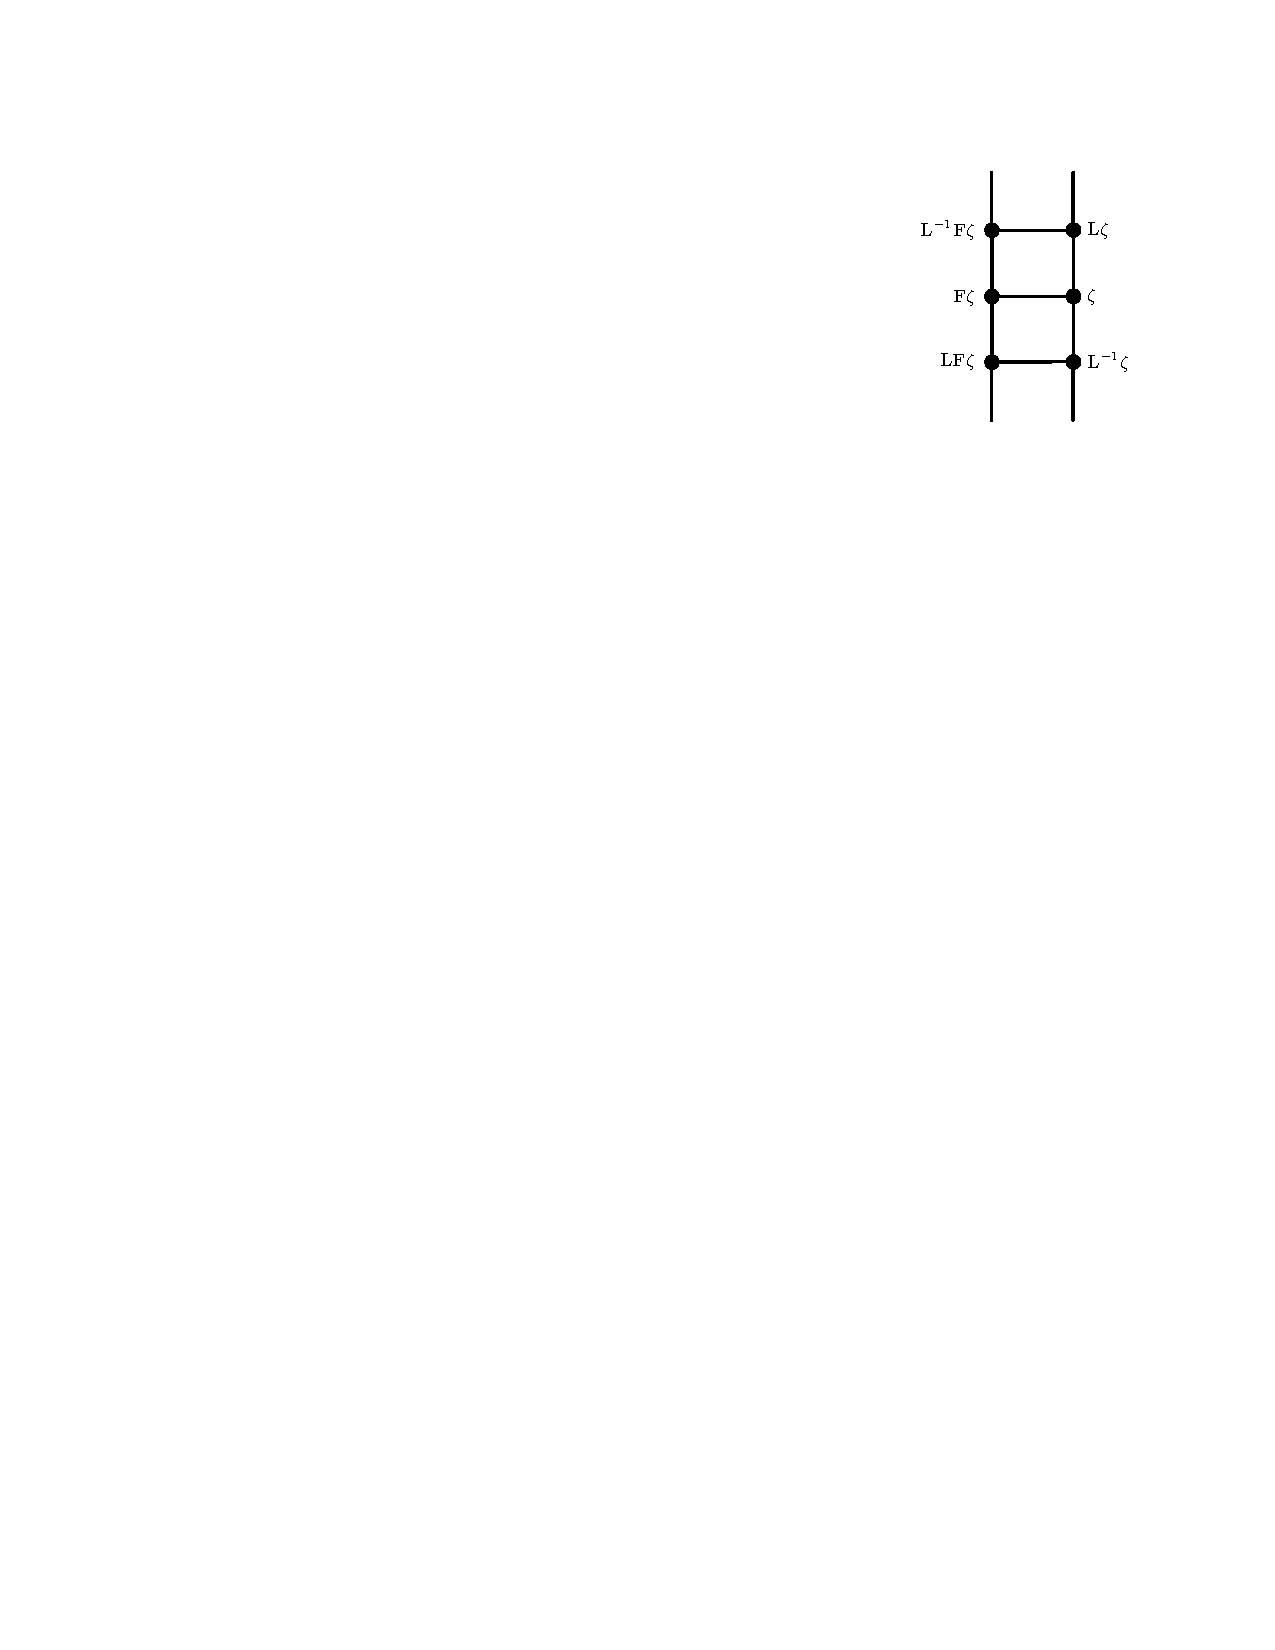
\includegraphics[width=0.5\textwidth]{ladder.pdf}
    \end{frame}

    \begin{frame}{The Operations}

        \begin{definition}
            $\op{R}\left\{\vec{q},\vec{p}\right\} = \left\{\vec{q}, \sqrt{1-\alpha}\vec{p} + \sqrt{\alpha}\vec{n}\right\}, \vec{n} \sim \norm\left(\vec{0}, \mat{M}\right)$ corrupts the momentum with noise. The $\alpha$~parameter determines by exactly how much.
        \end{definition}

        \vfill

        \centering
        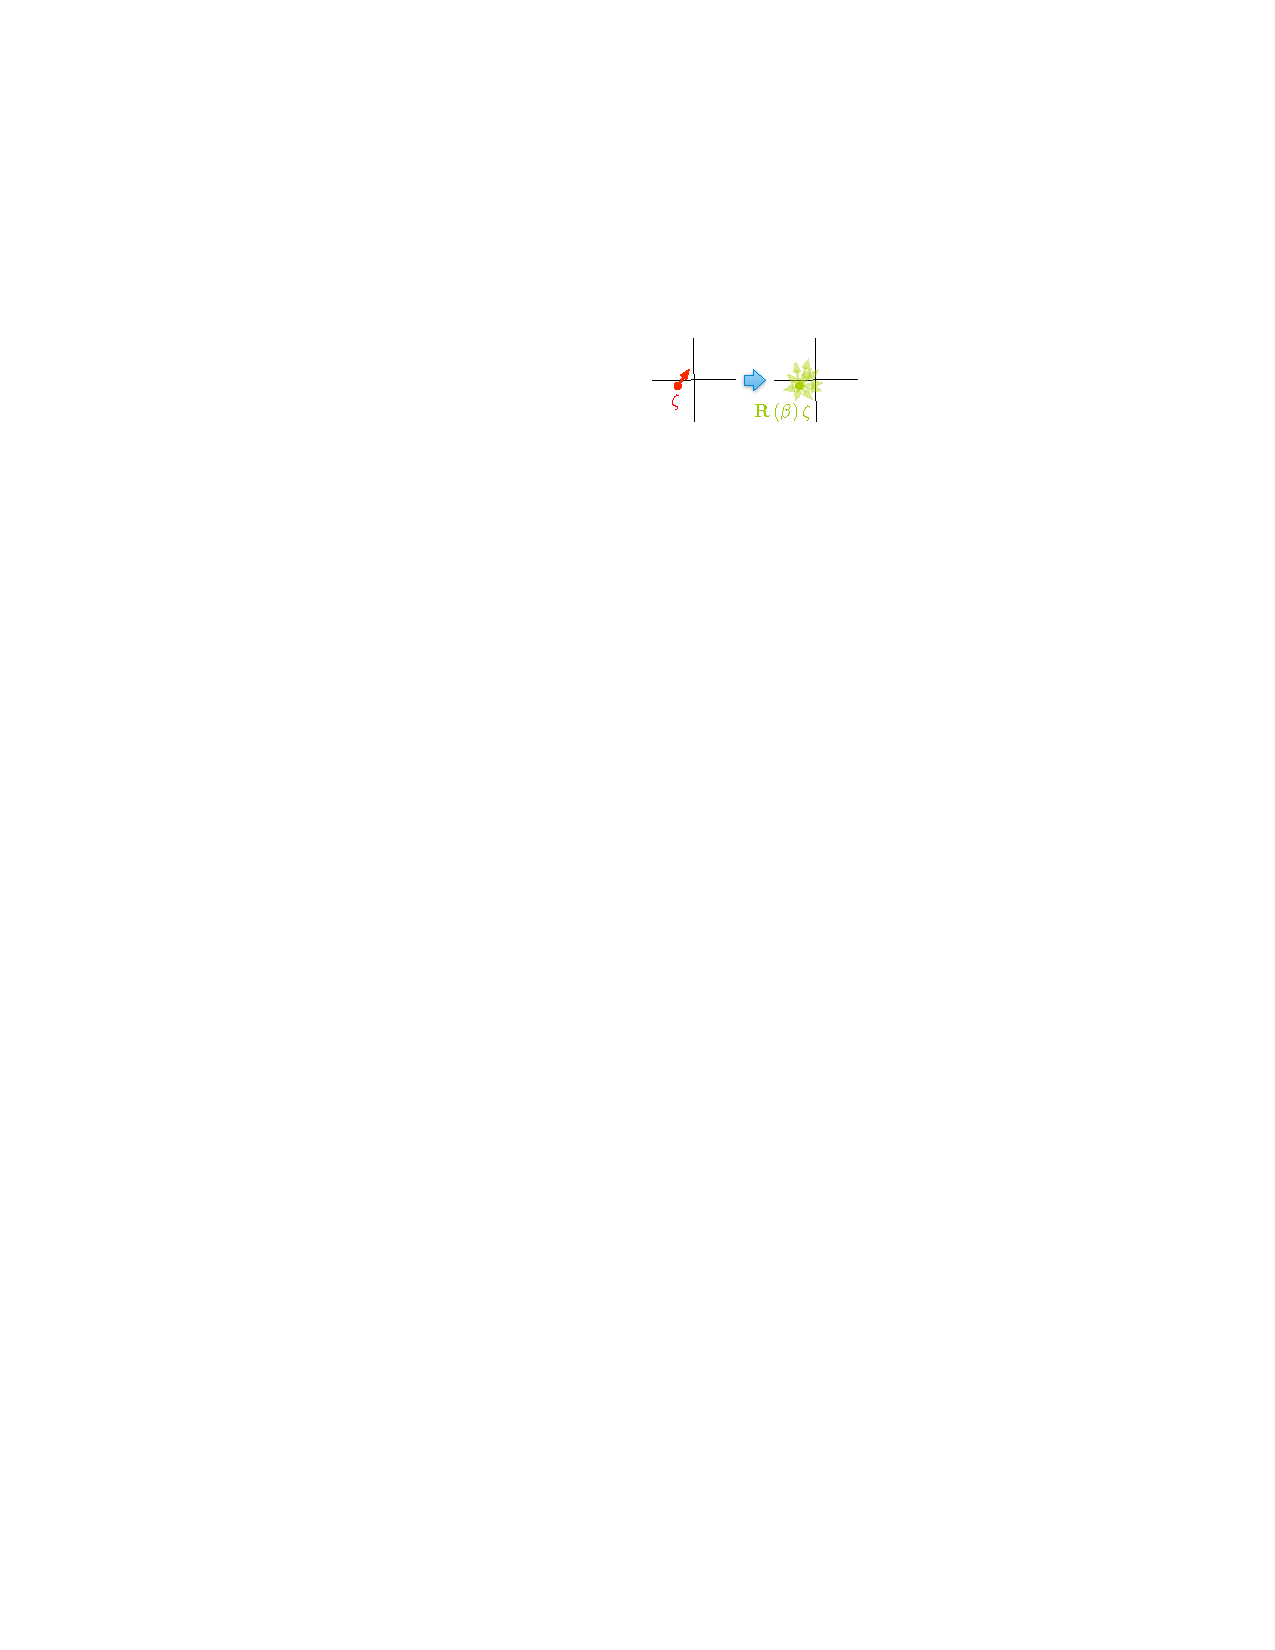
\includegraphics[width=0.75\textwidth]{R.pdf}

    \end{frame}

    \begin{frame}{The HMC Algorithm}
            \begin{algorithmic}[1]
            \Function {HamiltonUpdate}{$\left\{\vec{q},\vec{p}\right\}$}
                \State $\left\{\vec{q}^\prime, \vec{p}^\prime\right\}
                    \leftarrow \op{F}\op{L}\left\{\vec{q},\vec{p}\right\}$
                \State $a \leftarrow \min\left(1,
                    \exp\left(
                        H\left(\vec{q}, \vec{p}\right) - H\left(\vec{q}^\prime,
                            \vec{p}^\prime\right)\right)\right)$
                \State $\left\{\vec{q},\vec{p}\right\} \leftarrow
                    \begin{cases}
                        \left\{\vec{q}^\prime, \vec{p}^\prime\right\}
                            & \text{with probability } a \\
                        \left\{\vec{q},\vec{p}\right\}
                            & \text{with probability } 1 - a
                    \end{cases}$
                \State $\left\{\vec{q},\vec{p}\right\} \leftarrow
                            \op{R}\op{F}\left\{\vec{q},\vec{p}\right\}$
                \State \Return $\left\{\vec{q},\vec{p}\right\}$
            \EndFunction
            \end{algorithmic}
    \end{frame}

    \begin{frame}{Properties of HMC}
        \begin{itemize}
            \item Ergodic
            \item Optimal acceptance rate is $0.651$
            \item Scales on the order $d^\frac{5}{4}$
            \item Cannot update discrete parameters
            \item Can be mixed with other MCMC updates
        \end{itemize}
    \end{frame}

    \begin{frame}{Looks great for normal distributions!}
        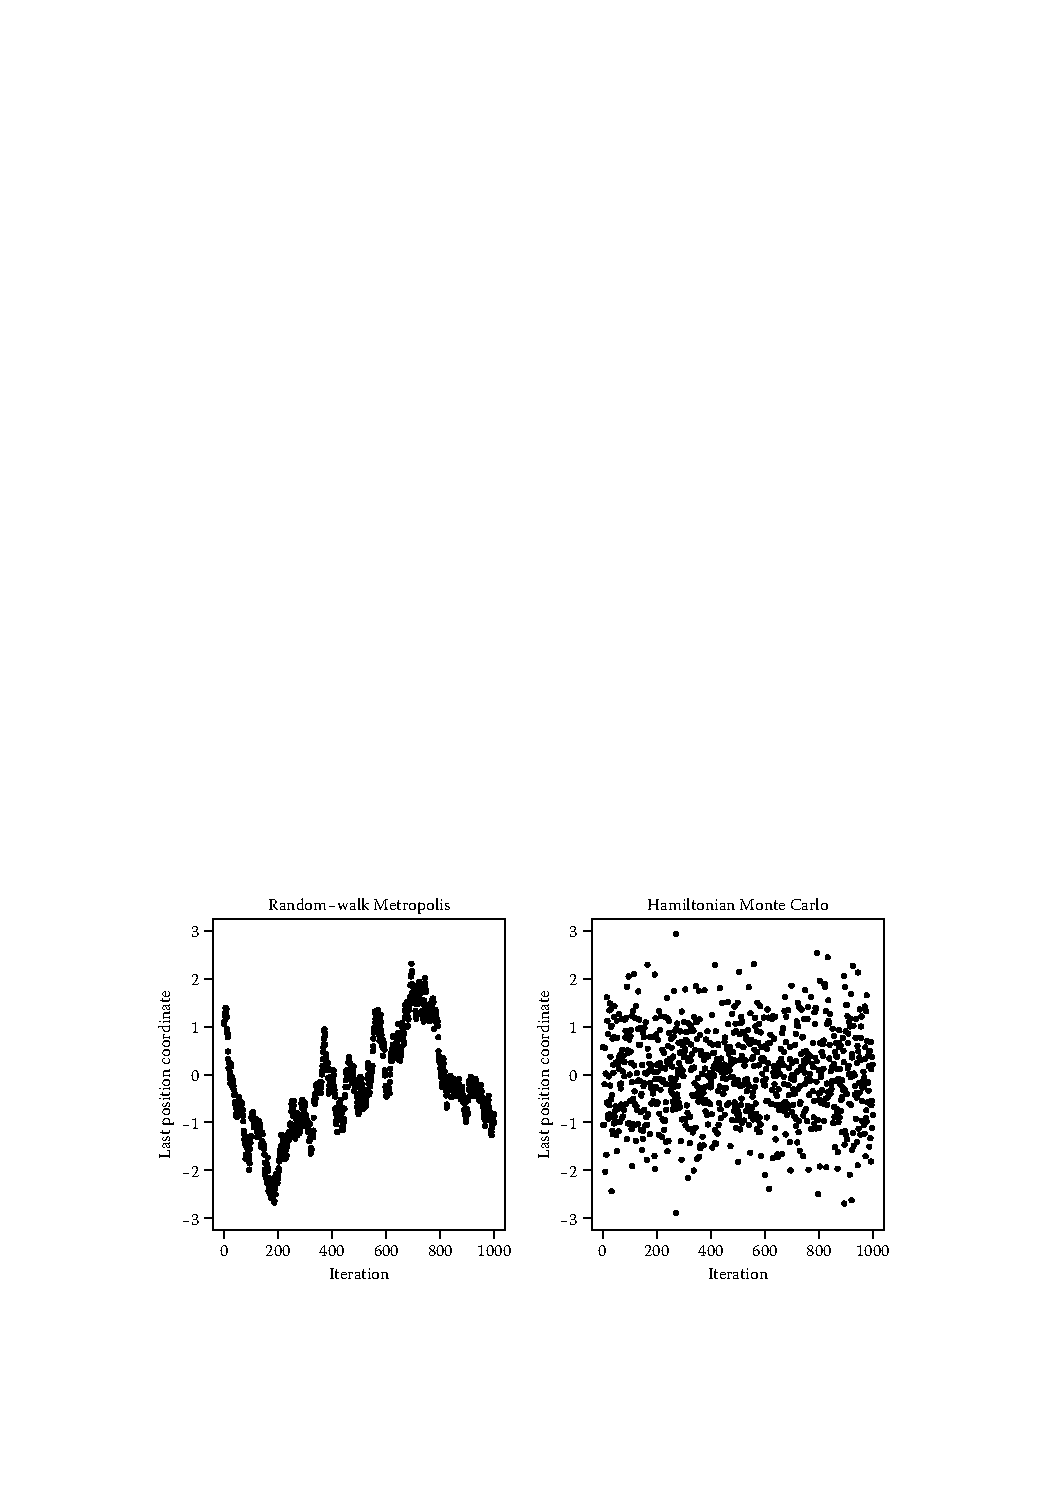
\includegraphics[width=\textwidth]{rw-vs-hmc.pdf}
    \end{frame}

    \begin{frame}{Looks great for normal distributions!}
        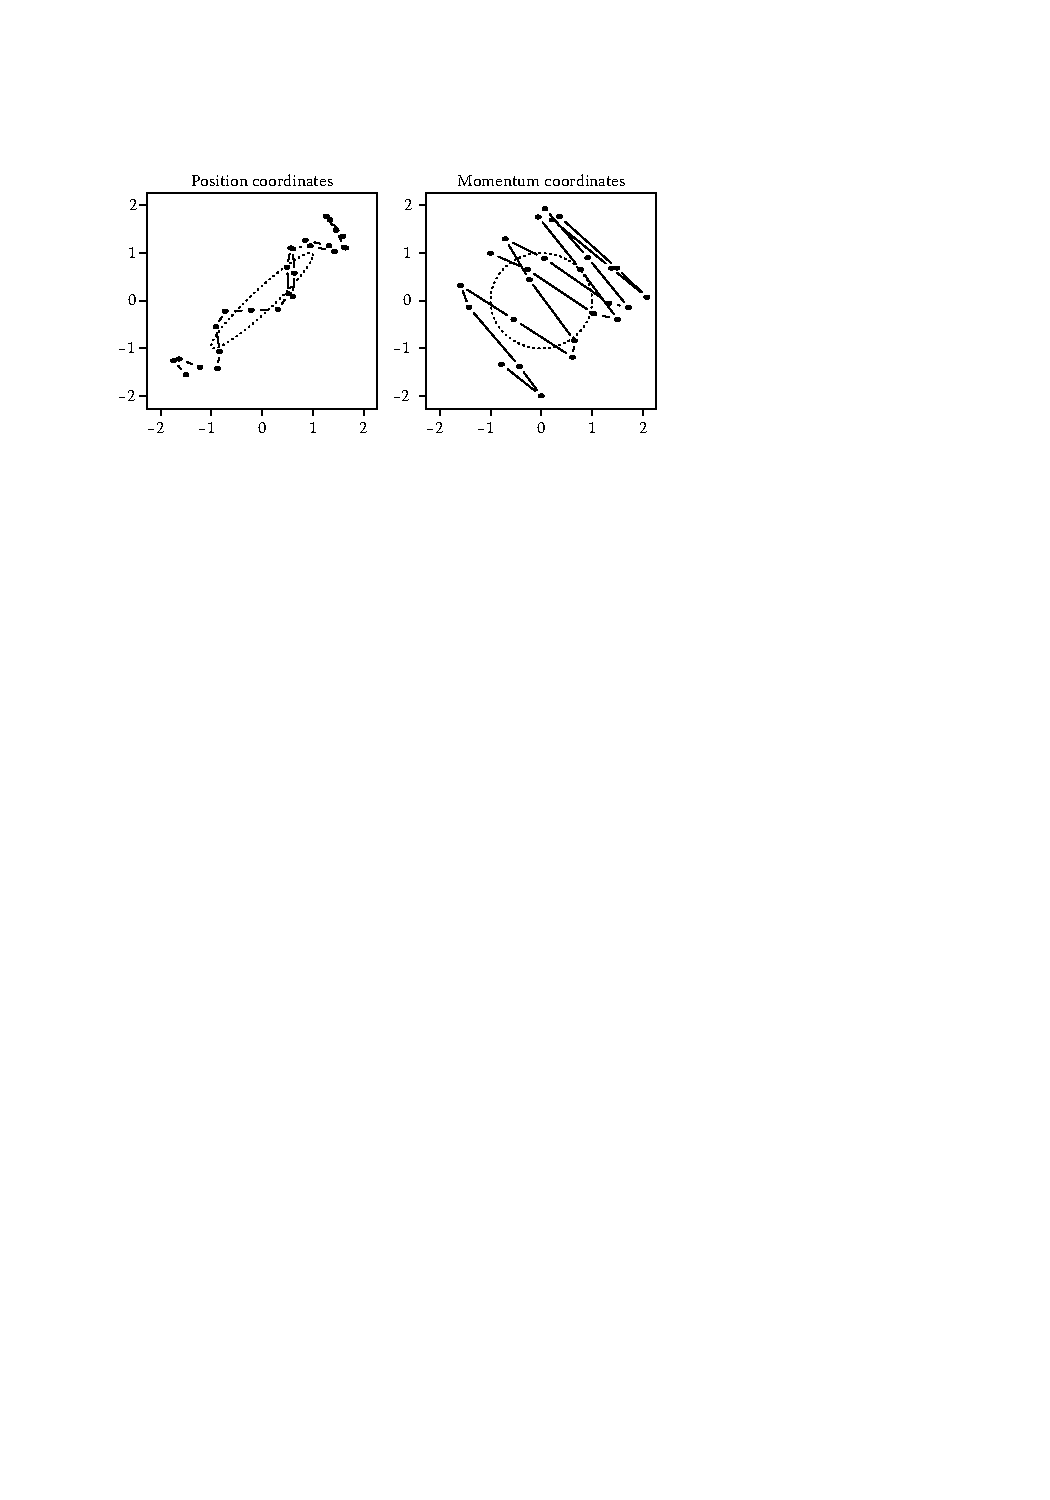
\includegraphics[width=\textwidth]{rw-vs-hmc2.pdf}
    \end{frame}

    \begin{frame}{In summary...}
        \textbf{Upgrading to HMC is like putting your MCMC through rehab and then giving it a pair of skis.}
        \vspace{12pt}
        \pause
        \begin{columns}[c]
            \begin{column}{0.5\textwidth}
                \centering
                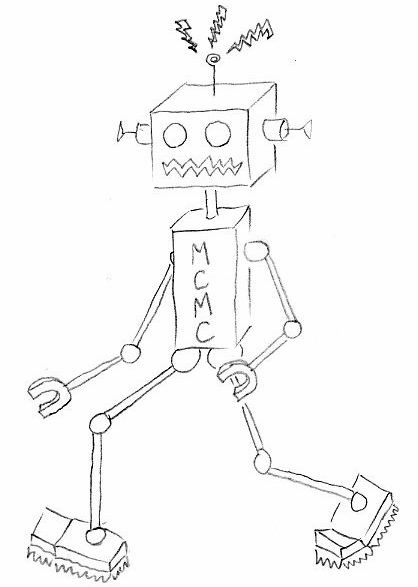
\includegraphics[width=0.5\textwidth]{mcmc-robot.jpg}
            \end{column}
            \pause
            \begin{column}{0.5\textwidth}
                \centering
                
\includegraphics[width=\textwidth]{hmc-robot.jpg}
            \end{column}
        \end{columns}

    \end{frame}

    \section{Implementation}

    \begin{frame}{Implementation}

        \begin{itemize}

            \item Implemented \texttt{HamiltonUpdate} as operator whose Hastings' ratio is given by difference in kinetic energy

            \item Constraints handled by ``bouncing''

            \item $\epsilon$ auto-optimised; all other tuning parameters fixed

            \item Added a high-level method signature \texttt{double~differentiate(Parameter param, int dim)}

            \item Things I have differentiated (and tested):
                \begin{itemize}
                    \item Base distributions and priors
                    \item Basic coalescent models
                    \item Birth--death--sampling model
                    \item Tree likelihood (including BEAGLE implementation)
                \end{itemize}

        \end{itemize}

    \end{frame}

    \begin{frame}{Differentiating the Felsenstein Tree Likelihood}

        The molecular substitution probabilities for time~$t$ are given by
        \begin{equation*}
            \mat{P}\left(t\right) = e^{\mat{Q}t} \implies \frac{\dd \mat{P}}{\dd t} = \mat{Q}e^{\mat{Q}t}
        \end{equation*}
        where $\mat{Q}$ is the instantaneous rate matrix.
        Therefore $\frac{\partial p\left(D\mid T\right)}{\partial b_i}$ is given by substituting differentiated matrix for original at the branch and running Felsenstein's pruning algorithm.
        Then then derivative with respect to node height $n_i$ is
        \begin{equation*}
            \frac{\partial p\left(D\mid T\right)}{\partial n_i} = - \frac{\partial p\left(D\mid T\right)}{\partial b_i} + \frac{\partial p\left(D\mid T\right)}{\partial b_{c_1}} + \frac{\partial p\left(D\mid T\right)}{\partial b_{c_2}}
        \end{equation*}
        where $c_1,c_2$ are children of $i$.
        Differentiate tree likelihood against branches in pre-order to maximise the utility of partials!

    \end{frame}

    \section{Results}

    \begin{frame}{Main Finding}
        \begin{itemize}
            \item For Bayesian phylogenetics, it is really hard to beat MCMC!
            \item Simulation study
            \begin{itemize}
                \item 32 taxa
                \item Constant-size coalescent
                \item 2048 bp alignment under HKY model
                \item Estimate node heights
            \end{itemize}
            \item Unrealistically-optimised HMC (but still not optimal)
            \item HMC nearly on par with MCMC as measured in ESS/time
            \item HMC has \emph{low} ACT (5--20) vs. MCMC (500+)
            \item All parameters mix about equally well for HMC
            \item Need to improve tuning scheme and look at larger/more difficult problems
        \end{itemize}
    \end{frame}

    % \begin{frame}
    %     Implementing derivatives for everything is really annoying but necessary.
    %
    %     \begin{lstlisting}
    %         public double logNodeProbability(Tree tree, NodeRef node) {
    %             final double height = tree.getNodeHeight(node);
    %             final double r = getR();
    %             final double mrh = -r * height;
    %             final double a = getA();
    %             final double rho = getRho();
    %
    %             if (conditionalOnRoot && tree.isRoot(node)) {
    %                 return (tree.getTaxonCount() - 2) * logConditioningTerm(height);
    %             }
    %
    %             final double z = Math.log(rho + ((1 - rho) - a) * Math.exp(mrh));
    %             double l = -2 * z + mrh;
    %
    %             if (!conditionOnOrigin && !conditionalOnRoot && tree.isRoot(node)) {
    %                 l += mrh - z;
    %             }
    %
    %             return l;
    %         }
    %     \end{lstlisting}
    % \end{frame}

    \begin{frame}{Potential extensions}

    \begin{block}{In the literature}
        \begin{itemize}
            \item NUTS (No-U-Turns Sampler)
            \item Look Ahead HMC
            \item Riemannian Manifold HMC
            \item Spherical HMC
            \item Wormhole HMC
        \end{itemize}
    \end{block}

    \begin{block}{From the group}
        \begin{itemize}
            \item Multivariate normal approximations
            \item Discrete energy-transitions
            \item Simultaneous tuning of multiple parameters
        \end{itemize}
    \end{block}

    \end{frame}

\end{document}